% --------------------------------------------------------------
% This is all preamble stuff that you don't have to worry about.
% Head down to where it says "Start here"
% --------------------------------------------------------------
 
\documentclass[12pt]{article}
 
\usepackage[margin=1in]{geometry} 
\usepackage{amsmath,amsthm,amssymb, fontspec}
\usepackage{tikz}
\usetikzlibrary{automata,positioning}
\newfontfamily{\C}{微軟正黑體}
\XeTeXlinebreaklocale "zh"
\XeTeXlinebreakskip = 0pt plus 1pt
 
\newcommand{\N}{\mathbb{N}}
\newcommand{\Z}{\mathbb{Z}}
 
\newenvironment{theorem}[2][Theorem]{\begin{trivlist}
\item[\hskip \labelsep {\bfseries #1}\hskip \labelsep {\bfseries #2.}]}{\end{trivlist}}
\newenvironment{lemma}[2][Lemma]{\begin{trivlist}
\item[\hskip \labelsep {\bfseries #1}\hskip \labelsep {\bfseries #2.}]}{\end{trivlist}}
\newenvironment{exercise}[2][Exercise]{\begin{trivlist}
\item[\hskip \labelsep {\bfseries #1}\hskip \labelsep {\bfseries #2.}]}{\end{trivlist}}
\newenvironment{problem}[2][Problem]{\begin{trivlist}
\item[\hskip \labelsep {\bfseries #1}\hskip \labelsep {\bfseries #2.}]}{\end{trivlist}}
\newenvironment{question}[2][Question]{\begin{trivlist}
\item[\hskip \labelsep {\bfseries #1}\hskip \labelsep {\bfseries #2.}]}{\end{trivlist}}
\newenvironment{corollary}[2][Corollary]{\begin{trivlist}
\item[\hskip \labelsep {\bfseries #1}\hskip \labelsep {\bfseries #2.}]}{\end{trivlist}}

\setlength\parindent{24pt}
 
\begin{document}
 
% --------------------------------------------------------------
%                         Start here
% --------------------------------------------------------------
 
\title{Homework 2}%replace X with the appropriate number
\author{\textnormal{\C{郝晉凱}}\\
B01705041 \textnormal{\C{資管三}}}
\maketitle
 
 
 
 
\begin{problem}{1}
\end{problem}
\begin{center}
    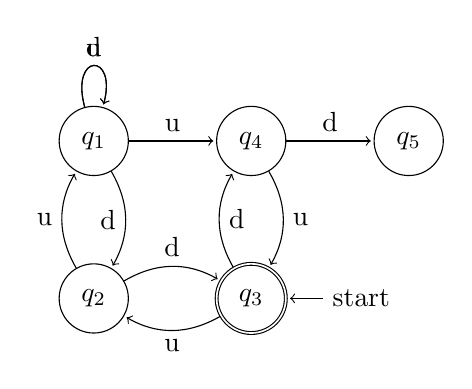
\begin{tikzpicture}[shorten >=1pt,node distance=2cm,on grid,auto] 
       \node[state] (q_1) {$q_1$}; 
       \node[state] (q_2) [below=of q_1] {$q_2$}; 
       \node[state, initial right, accepting] (q_3) [right=of q_2] {$q_3$};
       \node[state] (q_4) [right=of q_1] {$q_4$};
       \node[state] (q_5) [right=of q_4] {$q_5$};
        \path[->]
        		(q_1)		edge [loop above] node {u} ()
              		edge [bend left] node [left] {d} (q_2)
	    	(q_2)		edge [bend left] node [left] {u} (q_1)
              		edge [bend left] node [above] {d} (q_3)
     		(q_3)		edge [bend left] node [below] {u} (q_2)
              		edge [bend left] node [right] {d} (q_4)
	    	(q_4)		edge [bend left] node [right] {u} (q_3)
              		edge node {d} (q_5)
           	(q_1)		edge node {u} (q_4)
              		edge [loop above] node {d} ();	
    \end{tikzpicture} 
\end{center}


\begin{paragraph}
\newline
\end{paragraph}


\begin{problem}{2}
\end{problem}
\begin{enumerate}
	\item[a.] \hfill 
	\begin{center}
            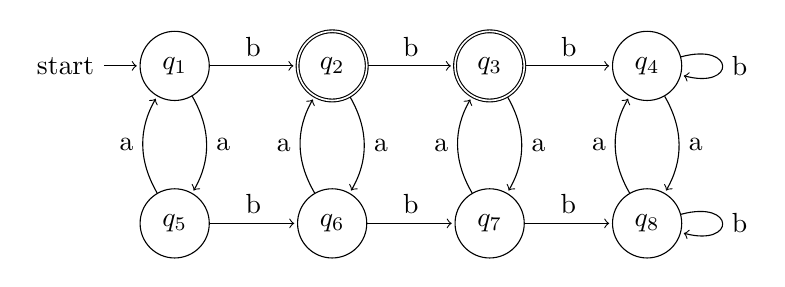
\begin{tikzpicture}[shorten >=1pt,node distance=2cm,on grid,auto] 
               \node[state, initial] (q_1) {$q_1$}; 
               \node[state, accepting] (q_2) [right=of q_1] {$q_2$}; 
               \node[state, accepting] (q_3) [right=of q_2] {$q_3$};
               \node[state] (q_4) [right=of q_3] {$q_4$};
               \node[state] (q_5) [below=of q_1] {$q_5$};
               \node[state] (q_6) [right=of q_5] {$q_6$};
               \node[state] (q_7) [right=of q_6] {$q_7$};
               \node[state] (q_8) [right=of q_7] {$q_8$};
		\path[->]
			(q_1)		edge [bend left] node [right] {a} (q_5)
					edge node {b} (q_2)
			(q_2)		edge [bend left] node [right] {a} (q_6)
					edge node {b} (q_3)
			(q_3)		edge [bend left] node [right] {a} (q_7)
					edge node {b} (q_4)
			(q_4)		edge [bend left] node [right] {a} (q_8)
					edge [loop right] node {b} ()
			(q_5)		edge [bend left] node [left] {a} (q_1)
					edge node {b} (q_6)
			(q_6)		edge [bend left] node [left] {a} (q_2)
					edge node {b} (q_7)
			(q_7)		edge [bend left] node [left] {a} (q_3)
					edge node {b} (q_8)
			(q_8)		edge [bend left] node [left] {a} (q_4)
					edge [loop right] node {b} ();
            \end{tikzpicture} 
        \end{center}
        
	\item[b.] \hfill 
	\begin{center}
            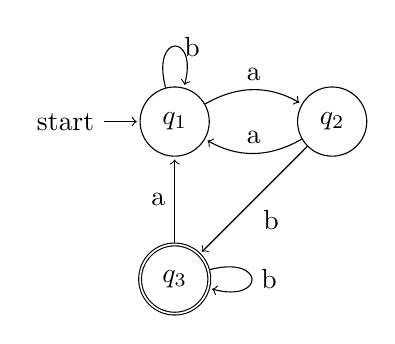
\begin{tikzpicture}[shorten >=1pt,node distance=2cm,on grid,auto] 
               \node[state, initial] (q_1) {$q_1$}; 
               \node[state] (q_2) [right=of q_1] {$q_2$}; 
               \node[state, accepting] (q_3) [below=of q_1] {$q_3$};
		\path[->]
			(q_1)		edge [loop above] node [right] {b} ()
					edge [bend left] node [above] {a} (q_2)
			(q_2)		edge [bend left] node [above] {a} (q_1)
					edge node {b} (q_3)
			(q_3)		edge node {a} (q_1)
					edge [loop right] node {b} ();
            \end{tikzpicture} 
        \end{center}
\end{enumerate}


\begin{paragraph}
\newline
\end{paragraph}


\begin{problem}{3}
\end{problem}
\begin{enumerate}
	\item[a.] \hfill 
	\begin{center}
            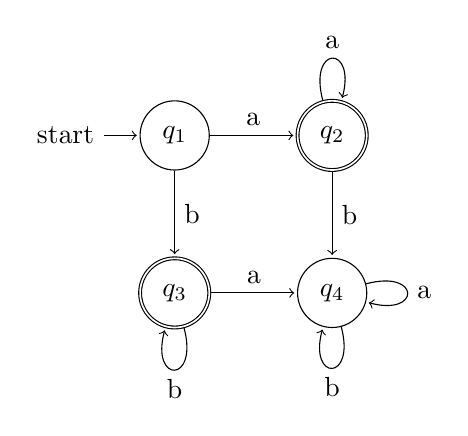
\begin{tikzpicture}[shorten >=1pt,node distance=2cm,on grid,auto] 
               \node[state, initial] (q_1) {$q_1$}; 
               \node[state, accepting] (q_2) [right=of q_1] {$q_2$}; 
               \node[state, accepting] (q_3) [below=of q_1] {$q_3$};
               \node[state] (q_4) [right=of q_3] {$q_4$};
		\path[->]
			(q_1)		edge node {a} (q_2)
					edge node {b} (q_3)
			(q_2)		edge [loop above] node {a} ()
					edge node {b} (q_4)
			(q_3)		edge [loop below] node {b} ()
					edge node {a} (q_4)
			(q_4)		edge [loop right] node {a} ()
					edge [loop below] node {b} ();
            \end{tikzpicture} 
        \end{center}
        
	\item[b.] \hfill 
	\begin{center}
            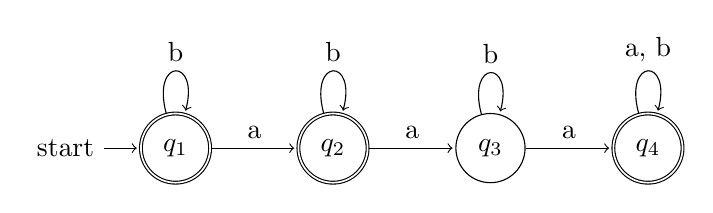
\begin{tikzpicture}[shorten >=1pt,node distance=2cm,on grid,auto] 
               \node[state, accepting, initial] (q_1) {$q_1$}; 
               \node[state, accepting] (q_2) [right=of q_1] {$q_2$}; 
               \node[state] (q_3) [right=of q_2] {$q_3$};
               \node[state, accepting] (q_4) [right=of q_3] {$q_4$};
		\path[->]
			(q_1)		edge [loop above] node {b} ()
					edge node {a} (q_2)
			(q_2)		edge [loop above] node {b} ()
					edge node {a} (q_3)
			(q_3)		edge [loop above] node {b} ()
					edge node {a} (q_4)
			(q_4)		edge [loop above] node {a, b} ();
            \end{tikzpicture} 
        \end{center}
\end{enumerate}


\begin{paragraph}
\newline
\end{paragraph}


\begin{problem}{4}
\end{problem}
\begin{enumerate}
	\item[a.] \hfill 
	\begin{center}
            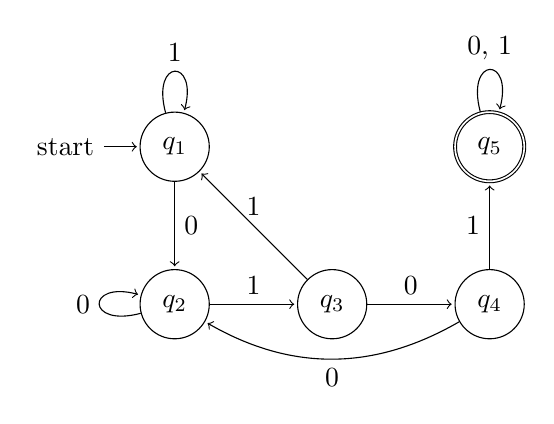
\begin{tikzpicture}[shorten >=1pt,node distance=2cm,on grid,auto] 
               \node[state, initial] (q_1) {$q_1$};                              
               \node[state] (q_2) [below=of q_1] {$q_2$};
               \node[state] (q_3) [right=of q_2] {$q_3$};
               \node[state] (q_4) [right=of q_3] {$q_4$};
               \node[state, accepting] (q_5) [above=of q_4] {$q_5$}; 
		\path[->]
			(q_1)		edge [loop above] node {1} ()
					edge node [right] {0} (q_2)
			(q_2)		edge node {1} (q_3)
					edge [loop left] node {0} ()
			(q_3)		edge node {0} (q_4)
					edge node [above] {1} (q_1)
			(q_4)		edge node {1} (q_5)
					edge [bend left] node [below] {0} (q_2)
			(q_5)		edge [loop above] node {0, 1} ();
            \end{tikzpicture} 
        \end{center}
        
	\item[b.] \hfill
	\begin{center}
            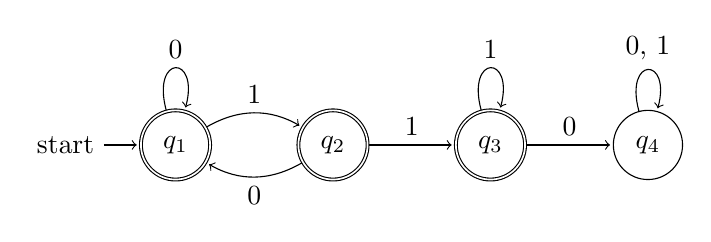
\begin{tikzpicture}[shorten >=1pt,node distance=2cm,on grid,auto] 
               \node[state, accepting, initial] (q_1) {$q_1$}; 
               \node[state, accepting] (q_2) [right=of q_1] {$q_2$}; 
               \node[state, accepting] (q_3) [right=of q_2] {$q_3$};
               \node[state] (q_4) [right=of q_3] {$q_4$};
		\path[->]
			(q_1)		edge [loop above] node {0} ()
					edge [bend left] node [above] {1} (q_2)
			(q_2)		edge [bend left] node [below] {0} (q_1)
					edge node {1} (q_3)
			(q_3)		edge [loop above] node {1} ()
					edge node {0} (q_4)
			(q_4)		edge [loop above] node {0, 1} ();
            \end{tikzpicture} 
        \end{center}
\end{enumerate}


\begin{paragraph}
\newline
\end{paragraph}


\begin{problem}{5}
\end{problem}
\begin{proof}
	\par Given $A_1 \cdot w \in A$ is regular. Then it's reverse $= w \cdot A_1^R$ is regular (the regular operation.) By induction, if $A$ is regular, $A^R$ is regular.
\end{proof}


\begin{paragraph}
\newline
\end{paragraph}


\begin{problem}{6}
\end{problem}
\begin{proof}
	\par Let $A = \left\{\begin{bmatrix} 0 \\ 0 \\ 0 \\ \end{bmatrix}, \begin{bmatrix} 0 \\ 1 \\ 1 \\ \end{bmatrix}, \begin{bmatrix} 1 \\ 0 \\ 1 \\ \end{bmatrix}\right\}$, $B = \left\{\begin{bmatrix} 1 \\ 1 \\ 0 \\ \end{bmatrix}\right\}$, $C = \left\{\begin{bmatrix} 0 \\ 0 \\ 1 \\ \end{bmatrix}\right\}$, and $D = \left\{\begin{bmatrix} 1 \\ 1 \\ 1 \\ \end{bmatrix}, \begin{bmatrix} 0 \\ 1 \\ 0 \\ \end{bmatrix}, \begin{bmatrix} 1 \\ 0 \\ 0 \\ \end{bmatrix}\right\}$. The state diagram for $B^R$ is as below. \\
	\begin{center}
            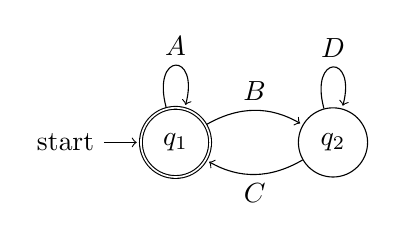
\begin{tikzpicture}[shorten >=1pt,node distance=2cm,on grid,auto] 
               \node[state, accepting, initial] (q_1) {$q_1$}; 
               \node[state] (q_2) [right=of q_1] {$q_2$}; 
		\path[->]
			(q_1)		edge [loop above] node {$A$} ()
					edge [bend left] node [above] {$B$} (q_2)
			(q_2)		edge [bend left] node [below] {$C$} (q_1)
					edge [loop above] node {$D$} ();
            \end{tikzpicture} 
        \end{center}
        \par Thus, $B^R$ is regular, by Problem 5, $B$ is regular.
\end{proof}


\begin{paragraph}
\newline
\end{paragraph}


\begin{problem}{7}
\end{problem}
\begin{proof}
	\par Let $\Sigma = \Sigma_1 \cup \Sigma_2$. Change $M_1 = (Q_1, \Sigma_1, \delta_1, q_1, F_1)$ and $M_2 = (Q_2, \Sigma_2, \delta_2, q_2, F_2)$ to $M_1 = (Q_1, \Sigma, \delta_1, q_1, F_1)$ and $M_2 = (Q_2, \Sigma, \delta_2, q_2, F_2)$ ,then do the proof like before.
\end{proof}
% --------------------------------------------------------------
%     You don't have to mess with anything below this line.
% --------------------------------------------------------------
\end{document}